\documentclass[tikz,border=5pt]{standalone}
\usepackage[UTF8]{ctex}
\usepackage{amsmath,amssymb,pgfplots}
\pgfplotsset{compat=1.18}
\usetikzlibrary{arrows.meta,calc}
\tikzset{>=Stealth,line cap=round,line join=round,
river/.style={fill=blue!7},landpath/.style={green!45!black,very thick},
swimpath/.style={blue!75!black,very thick},aux/.style={gray!60,dashed,thin},
dim/.style={gray!75,<->,thin},water/.style={blue!60!black,thick},
point/.style={circle,fill=black,inner sep=1.5pt}}
\newcommand{\banks}{
\fill[river](-2.3,0)rectangle(2.3,1);
\draw[thick](-2.3,0)--(2.3,0);
\draw[thick](-2.3,1)--(2.3,1);
}
\begin{document}
% 1. Plan view; the candidate path is not asserted to be optimal.
\begin{tikzpicture}[x=1.65cm,y=1.65cm,font=\small]
\banks
\coordinate(A)at(0,-1);\coordinate(B)at(0,2);
\coordinate(C)at(-.75,0);\coordinate(D)at(.75,1);
\draw[aux](A)--(B);
\draw[landpath,->](A)--(C);
\draw[swimpath,->](C)--(D);
\draw[landpath,->](D)--(B);
\foreach \p in {A,B,C,D}{\node[point]at(\p){};}
\node[below]at(A){$A$};\node[above]at(B){$B$};
\node[below left]at(C){$C$};\node[above right]at(D){$D$};
\node[below]at(-1.85,0){近岸};\node[above]at(-1.85,1){远岸};
\draw[water,->](.95,.45)--(1.85,.45)node[midway,above]{$v_0$};
\foreach \y in {-1,0,1,2}{\draw[gray!60,thin](2.45,\y)--(2.72,\y);}
\foreach \lo/\hi in {-1/0,0/1,1/2}{
\draw[dim](2.60,\lo)--(2.60,\hi)node[midway,right,text=black]{$h$};}
\draw[->](-2.05,-1.15)--(-1.40,-1.15)node[right]{$x$};
\draw[->](-2.05,-1.15)--(-2.05,-.53)node[above]{$y$};
\node at(0,-1.56){陆地速率 $v_1$；相对水速率 $v_1$};
\end{tikzpicture}
% 2. Exact optimized velocity triangle; alpha is relative to upstream.
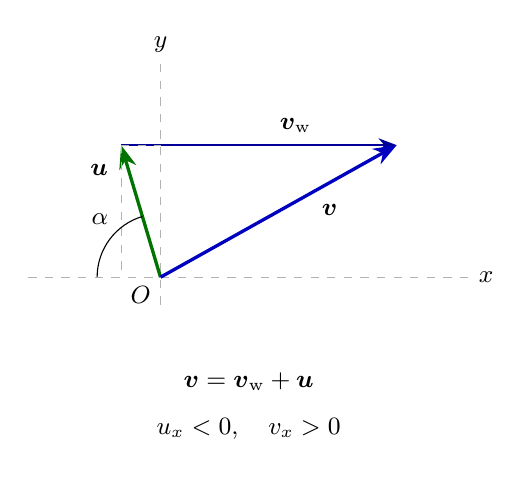
\begin{tikzpicture}[x=3.5cm,y=3.5cm,font=\small]
\coordinate(O)at(0,0);\coordinate(U)at(-.142857,.479157);
\coordinate(V)at(.857143,.479157);
\draw[aux](-.48,0)--(1.12,0)node[right,text=black]{$x$};
\draw[aux](0,-.10)--(0,.78)node[above,text=black]{$y$};
\draw[green!45!black,very thick,->](O)--(U);
\draw[water,->](U)--(V);
\draw[swimpath,->](O)--(V);
\draw[aux](U)--(-.142857,0);
\draw[aux](U)--(0,.479157);
\draw[thin](-.23,0)arc(180:106.60155:.23);
\node at(-.22,.21){$\alpha$};
\node[left]at(-.155,.39){$\boldsymbol u$};
\node[above]at(.49,.49){$\boldsymbol v_{\mathrm w}$};
\node[below right]at(.55,.30){$\boldsymbol v$};
\node[below left]at(O){$O$};
\node at(.32,-.38){$\boldsymbol v=\boldsymbol v_{\mathrm w}+\boldsymbol u$};
\node at(.32,-.55){$u_x<0,\quad v_x>0$};
\end{tikzpicture}
% 3. Translate DB to CE; E=(-d,h), not a spurious reflected point.
\begin{tikzpicture}[font=\small]
\begin{scope}[x=1.50cm,y=1.50cm]
\fill[river](-1.8,0)rectangle(1.8,1);
\draw[thick](-1.8,0)--(1.8,0);\draw[thick](-1.8,1)--(1.8,1);
\coordinate(A)at(0,-1);\coordinate(B)at(0,2);
\coordinate(C)at(-.894427,0);\coordinate(D)at(.894427,1);
\draw[landpath,->](A)--(C);\draw[swimpath,->](C)--(D);
\draw[landpath,->](D)--(B);
\foreach \p in {A,B,C,D}{\node[point]at(\p){};}
\node[below]at(A){$A$};\node[above]at(B){$B$};
\node[below left]at(C){$C$};\node[above right]at(D){$D$};
\draw[aux](C)--(-.894427,.5);\draw[aux](D)--(.894427,.5);
\draw[dim](-.894427,.5)--(.894427,.5)node[midway,above,text=black]{$d$};
\node at(0,2.50){实际三段路线};
\end{scope}
\begin{scope}[xshift=7cm,x=1.50cm,y=1.50cm]
\coordinate(A)at(0,-1);\coordinate(C)at(-.894427,0);
\coordinate(E)at(-1.788854,1);
\draw[aux](-2.1,0)--(.45,0);
\draw[gray!70,thin](A)--(E);
\draw[landpath,->](A)--(C);\draw[landpath,->](C)--(E);
\foreach \p in {A,C,E}{\node[point]at(\p){};}
\node[below right]at(A){$A$};\node[above right,xshift=2pt,yshift=2pt]at(C){$C$};
\node[above left]at(E){$E$};
\draw[aux](0,-1)--(.45,-1);\draw[aux](-1.788854,1)--(.45,1);
\draw[dim](.32,-1)--(.32,1)node[midway,right,text=black]{$2h$};
\draw[aux](-1.788854,1)--(-1.788854,1.65);
\draw[aux](0,-1)--(0,1.65);
\draw[dim](-1.788854,1.52)--(0,1.52)node[midway,above,text=black]{$d$};
\node at(-.8,2.50){平移 $DB$ 为 $CE$};
\node at(-.8,-1.57){取等：$A,C,E$ 共线};
\end{scope}
\end{tikzpicture}
% 4. A visible total-time minimum plus separate phase-time panel.
\begin{tikzpicture}[font=\small]
\begin{axis}[width=6.0cm,height=5.2cm,xmin=2,xmax=4.05,ymin=7.2,ymax=10.2,
axis lines=left,xlabel={$\tau=v_0t_{\mathrm s}/h$},ylabel={$\mathcal T=v_0T/h$},
xtick={2,2.5,3,3.5,4},ytick={7.5,8,9,10},samples=250,
tick label style={font=\scriptsize},label style={font=\small}]
\addplot[swimpath,domain=2:4.05]{x+2*sqrt(4+(x-.5*sqrt(max(0,x*x-4)))^2)};
\addplot[only marks,mark=*,mark size=1.7pt]coordinates{(2.086996779,7.453559925)};
\draw[thin,->](axis cs:2.8,7.82)--(axis cs:2.10,7.47);
\node[anchor=west,font=\scriptsize]at(axis cs:2.63,7.95){$\mathcal T_{\min}=10\sqrt5/3$};
\end{axis}
\begin{axis}[at={(6.5cm,0)},anchor=south west,width=5.8cm,height=5.2cm,
xmin=2,xmax=4.05,ymin=0,ymax=7,axis lines=left,
xlabel={$\tau$},ylabel={阶段时间 $\times v_0/h$},
xtick={2,3,4},ytick={0,2,4,6},samples=250,
tick label style={font=\scriptsize},label style={font=\small}]
\addplot[water,domain=2:4.05]{x};
\addplot[landpath,domain=2:4.05]{2*sqrt(4+(x-.5*sqrt(max(0,x*x-4)))^2)};
\node[font=\scriptsize,text=blue!60!black]at(axis cs:3.15,2.6){水中 $\tau$};
\node[font=\scriptsize,text=green!45!black]at(axis cs:3.05,6.55){两段陆地};
\end{axis}
\end{tikzpicture}
% 5. Normal escape, with a separate y-versus-time bound.
\begin{tikzpicture}[font=\small]
\begin{scope}[x=1.3cm,y=1.3cm]
\fill[river](-1.4,0)rectangle(1.4,1);
\draw[thick](-1.4,0)--(1.4,0);\draw[thick](-1.4,1)--(1.4,1);
\node[point]at(0,-1){};\node[below]at(0,-1){$A$};
\node[point]at(0,2){};\node[left]at(0,2){$B$};
\draw[red!75!black,very thick,->](0,2)--(0,3.2)node[right]{$v_2$};
\draw[water,->](-1,.5)--(.2,.5)node[midway,above]{$v_0$};
\node at(0,3.65){远离河岸逃跑};
\end{scope}
\begin{scope}[xshift=5.6cm]
\draw[->](-.3,0)--(4.7,0)node[right]{$t$};
\draw[->](0,-1.2)--(0,3.8)node[above]{$y$};
\draw[red!75!black,very thick](0,2)--(4,3.4);
\draw[swimpath](0,-1)--(4,.4);
\draw[dim](3.4,.19)--(3.4,3.19)node[midway,right,text=black]{$3h$};
\node[above]at(2.5,2.875){$2h+v_1t$};
\node[below]at(2.2,-.23){$-h+v_1t$};
\node[left]at(0,2){$2h$};\node[left]at(0,-1){$-h$};
\node at(2.3,4.35){临界 $v_2=v_1$：竖直间距始终为正};
\node at(2.3,-1.7){蓝线是追赶者的上界，不是实际路线};
\end{scope}
\end{tikzpicture}
% 6. A scaled exact counterexample: w=1/2, swim time=5/2, total=13/2.
\begin{tikzpicture}[x=1.65cm,y=1.65cm,font=\small]
\fill[river](-.7,0)rectangle(4.05,1);
\draw[thick](-.7,0)--(4.05,0);\draw[thick](-.7,1)--(4.05,1);
\coordinate(A)at(0,-1);\coordinate(C)at(0,0);
\coordinate(D)at(3.25,1);\coordinate(K)at(3.25,2);
\coordinate(B)at(0,2);
\draw[landpath,->](A)--(C);
\draw[swimpath,->](C)--(D);
\draw[landpath,->](D)--(K);
\draw[red!75!black,very thick,->](B)--(K);
\foreach \p in {A,B,C,D,K}{\node[point]at(\p){};}
\node[below]at(A){$A$};\node[below left]at(C){$C$};
\node[below right]at(D){$D$};\node[above]at(B){$B$};
\node[above right]at(K){截获点};
\node[above]at(1.4,2){猪沿下游跑};
\draw[water,->](2.0,.17)--(2.9,.17)node[midway,above]{$v_0$};
\node at(1.7,-1.48){$v_2=v_0/2,\quad T=13h/(2v_0),\quad x=13h/4$};
\end{tikzpicture}
\end{document}
